
\section{Neural Networks (50 Points) (Zhiting)}

\subsection{Neural network for regression}

Figure.\ref{nn} shows a two-layer neural network which learns a function $f:X\to Y$ where $X=(X_1, X_2) \in \mathbb{R}^2$. The weights $\bm{w} = \{w_1, \dots, w_6\}$ can be arbitrary. There are two possible choices for the function implemented by each unit in this network:
    \begin{itemize}
    \item S: signed sigmoid function $S(a) = sign[\sigma(a) - 0.5] = sign[\frac{1}{1+\exp\{-a\}}-0.5]$
    \item L: linear function $L(a) = ca$
    \end{itemize}
    where in both cases $a = \sum_i w_i X_i$.
    \begin{enumerate}
    \item Assign proper activation functions (S or L) to each unit in Figure.\ref{nn} so this neural network simulates a linear regression: $Y=\beta_1 X_1 + \beta_2 X_2$.
    \item Assign proper activation functions (S or L) for each unit in Figure.\ref{nn} so this neural network simulates a binary logistic regression classifier: $Y=\arg\max_{y}P(Y=y|X)$, where $P(Y=1|X) = \frac{\exp(\beta_1X_1+\beta_2X_2)}{1+\exp(\beta_1X_1+\beta_2X_2)}$, and $P(Y=-1|X) = \frac{1}{1+\exp(\beta_1X_1+\beta_2X_2)}$. Derive $\beta_1$ and $\beta_2$ in terms of $w_1,\dots,w_6$. \label{prob:p-nn-act-2}
    \item Assign proper activation functions (S or L) to each unit in Figure.\ref{nn} so this neural network simulates a boosting classifier which combines two logistic regression classifiers, $f_1: X\to Y_1$ and $f_2: X\to Y_2$, to produce its final prediction: $Y=sign[\alpha_1Y_1 + \alpha_2 Y_2]$. Use the same distribution in problem~1.1.\ref{prob:p-nn-act-2} for $f_1$ and $f_2$. Derive $\alpha_1$ and $\alpha_2$ in terms of $w_1,\dots,w_6$.
    \end{enumerate}

\begin{figure}[!htp]
  \centering
  % Requires \usepackage{graphicx}
  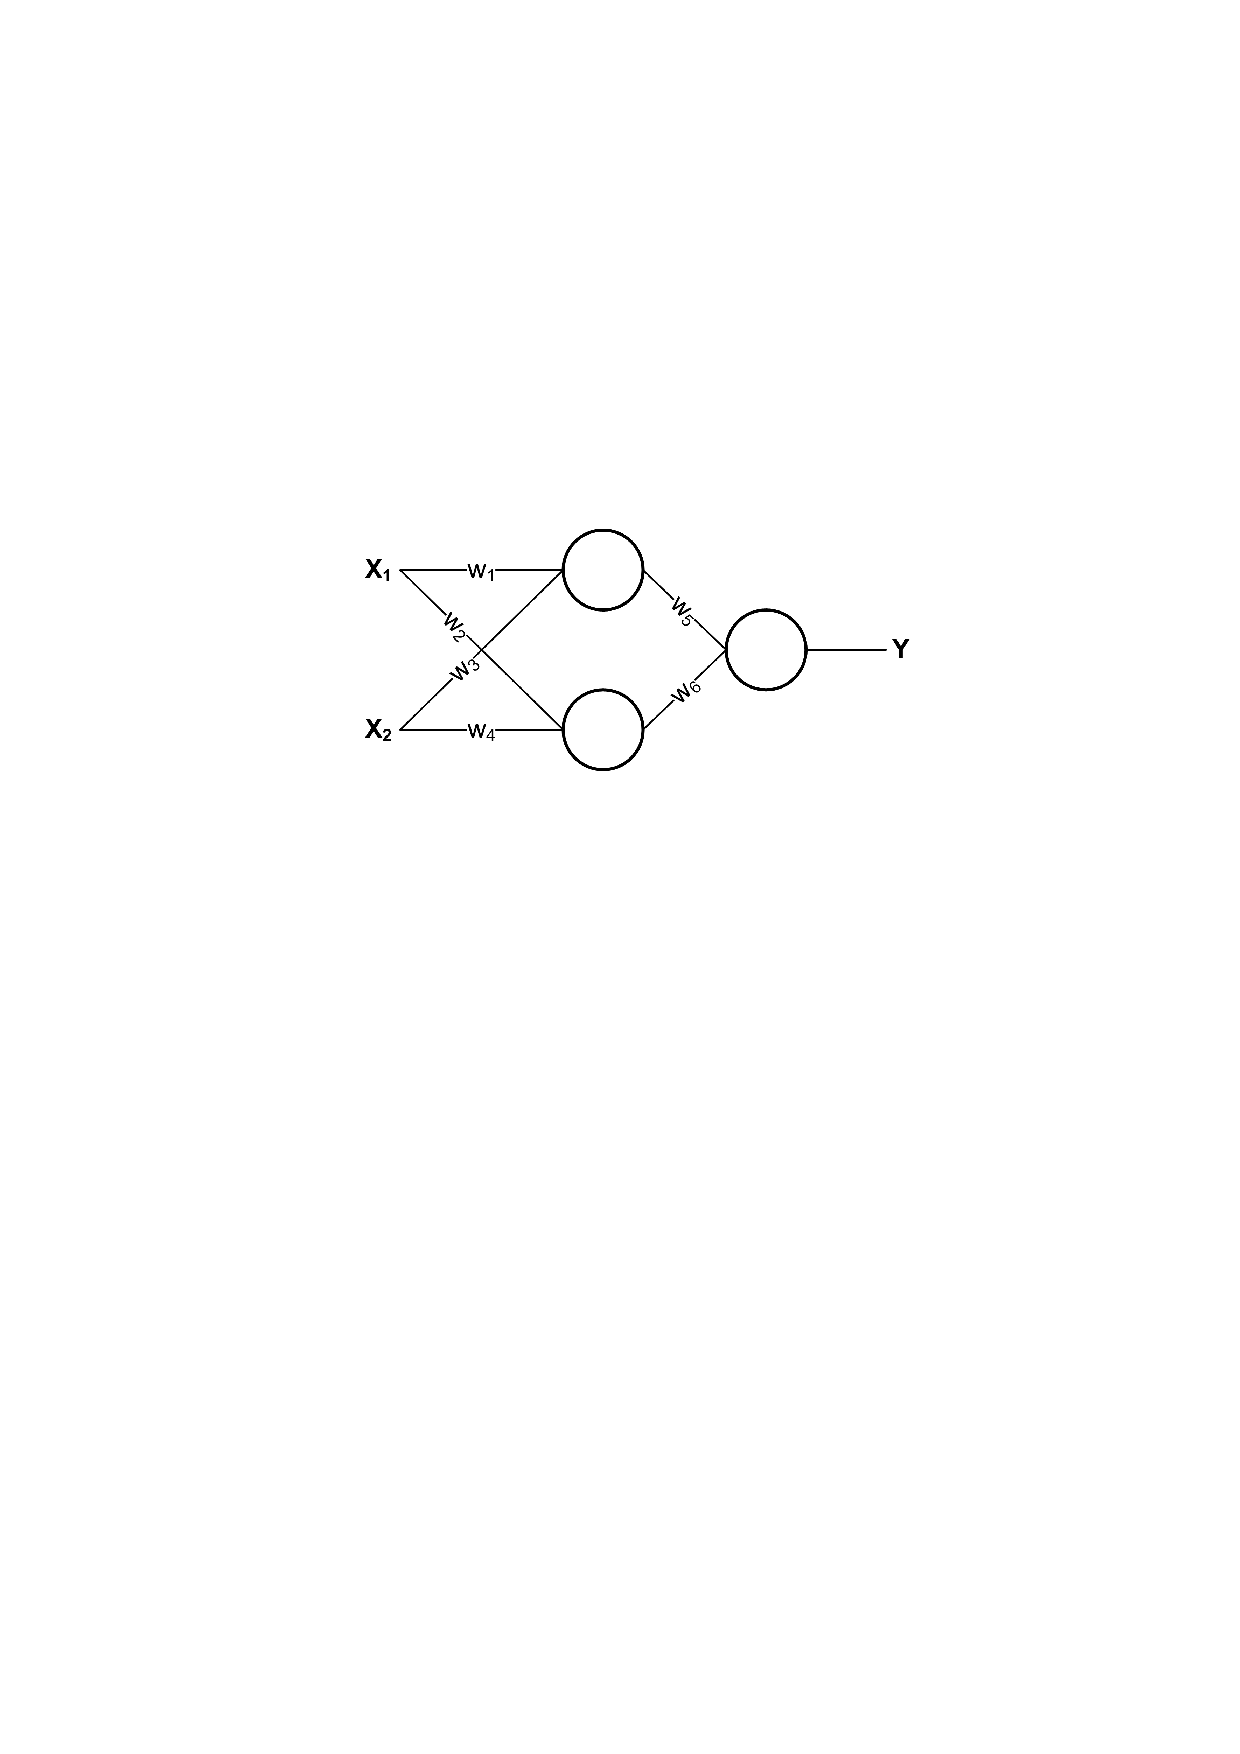
\includegraphics[width=0.5\textwidth]{Figure/nn}\\
  \caption{A two-layer neural network.}\label{nn}
\end{figure}

\subsection{Convolutional neural networks}

\begin{enumerate}
\item Count the total number of parameters in LeNet (pp.46, slides of Lecture.8). How many parameters in all of the convolutional layers? How many parameters in all of the fully-connected layers?
    
    {\color{red} 
    Note:
    \begin{enumerate}
    \item The filter size of each convolutional and pooling(subsampling) layer: \\
    %
    C1: $5\times 5$ (i.e., each unit of C1 has a $5\times 5$ receptive field in its preceding layer);\\
    S2: $2\times 2$;\\
    C3: $5\times 5$;\\
    S4: $2\times 2$;
    \item Fully-connected layers in LeNet include C5, F6, and OUTPUT
    \end{enumerate}
    }

\item In a convolutional layer the units are organized into planes, each of which is called a feature map. The units within a feature map (indexed $q$) have different inputs, but all share a common weight vector, $\bm{w}^{(q)}$. A convolutional network is usually trained through backprorogation. Let $J^{(q)}$ be the number of units in the $q$th feature map, $z_{j}^{(q)}$ the activation of the $j$th unit, $x_{ji}^{(q)}$ the $i$th input for the $j$th unit, $w_i^{(q)}$ the $i$th element of $\bm{w}^{(q)}$, $L$ the training loss. Derive the gradient of $w_{i}^{(q)}$.
\end{enumerate}

\subsection{Gradient vanishing/explosion}

In this problem we will study the difficulty of back-propagation in training deep neural networks. For simplicity, we consider the simplest deep neural network: one with just a single neuron in each layer, where the output of the neuron in the $j$th layer is $z_j = \sigma(a_j) = \sigma(w_jz_{j-1}+b_j)$. Here $\sigma$ is some activation function whose derivative on $x$ is $\sigma'(x)$. Let $m$ be the number of layers in the neural network, $L$ the training loss.

\begin{enumerate}
\item Derive the derivative of $L$ w.r.t. $b_1$ (the bias of the neuron in the first layer).
\item Assume the activation function is the usual sigmoid function $\sigma(x) = 1/(1+\exp\{-x\})$. The weights $\bm{w}$ are initialized to be $|w_j| < 1\ (j=1,\dots,m)$.
    \begin{enumerate}
    \item Explain why the above gradient ($\partial L/\partial b_1$) tends to vanish ($\to 0$) when $m$ is large.
    \item Even if $|w|$ is large, the above gradient would also tend to vanish, rather than explode ($\to\infty$). Explain why. (A rigorous proof is not required.)
    \end{enumerate}
\item One of the approaches to (partially) address the gradient vanishing/explosion problem is to use the rectified linear (ReL) activation function instead of the sigmoid. The ReL activation function is $\sigma(x) = \max\{0, x\}$. Explain why ReL can alleviate the gradient vanishing problem as faced by sigmoid.
\item A second approach to (partially) address the gradient vanishing/explosion problem is layer-wise pre-training. Restricted Boltzemann machine (RBM) is one of the widely-used models for layer-wise pre-training. Figure~\ref{rbm} shows an example of RBM which includes $K$ hidden units $\bm{h}$, and $J$ input units $\bm{v}$. Let us define the joint distribution as the following general form:
\begin{align}
P(\bm{v}, \bm{h}) = \frac{1}{Z}\exp\left( \sum_{i}\theta_{i}\phi_{i}(\bm{v},\bm{h}) \right),
\end{align}
where $Z=\sum_{\bm{v},\bm{h}}\exp\left( \sum_{i}\theta_{i}\phi_{i}(\bm{v},\bm{h}) \right)$ is the normalization term; $\phi_{i}(\bm{v},\bm{h})$ are some features; $\theta_{i}$ are the parameters corresponding to the weights in the RBM. Consider the simplest learning algorithm, gradient descent. Show that
\begin{align}
\frac{\partial \log P(\bm{v})}{\partial \theta_{i}} = \sum_{\bm{h}}\phi_{i}(\bm{v},\bm{h})P(\bm{h}|\bm{v}) - \sum_{\bm{v},\bm{h}}\phi_{i}(\bm{v},\bm{h})P(\bm{v},\bm{h}).
\end{align}
\end{enumerate}

\begin{figure}[!htp]
  \centering
  % Requires \usepackage{graphicx}
  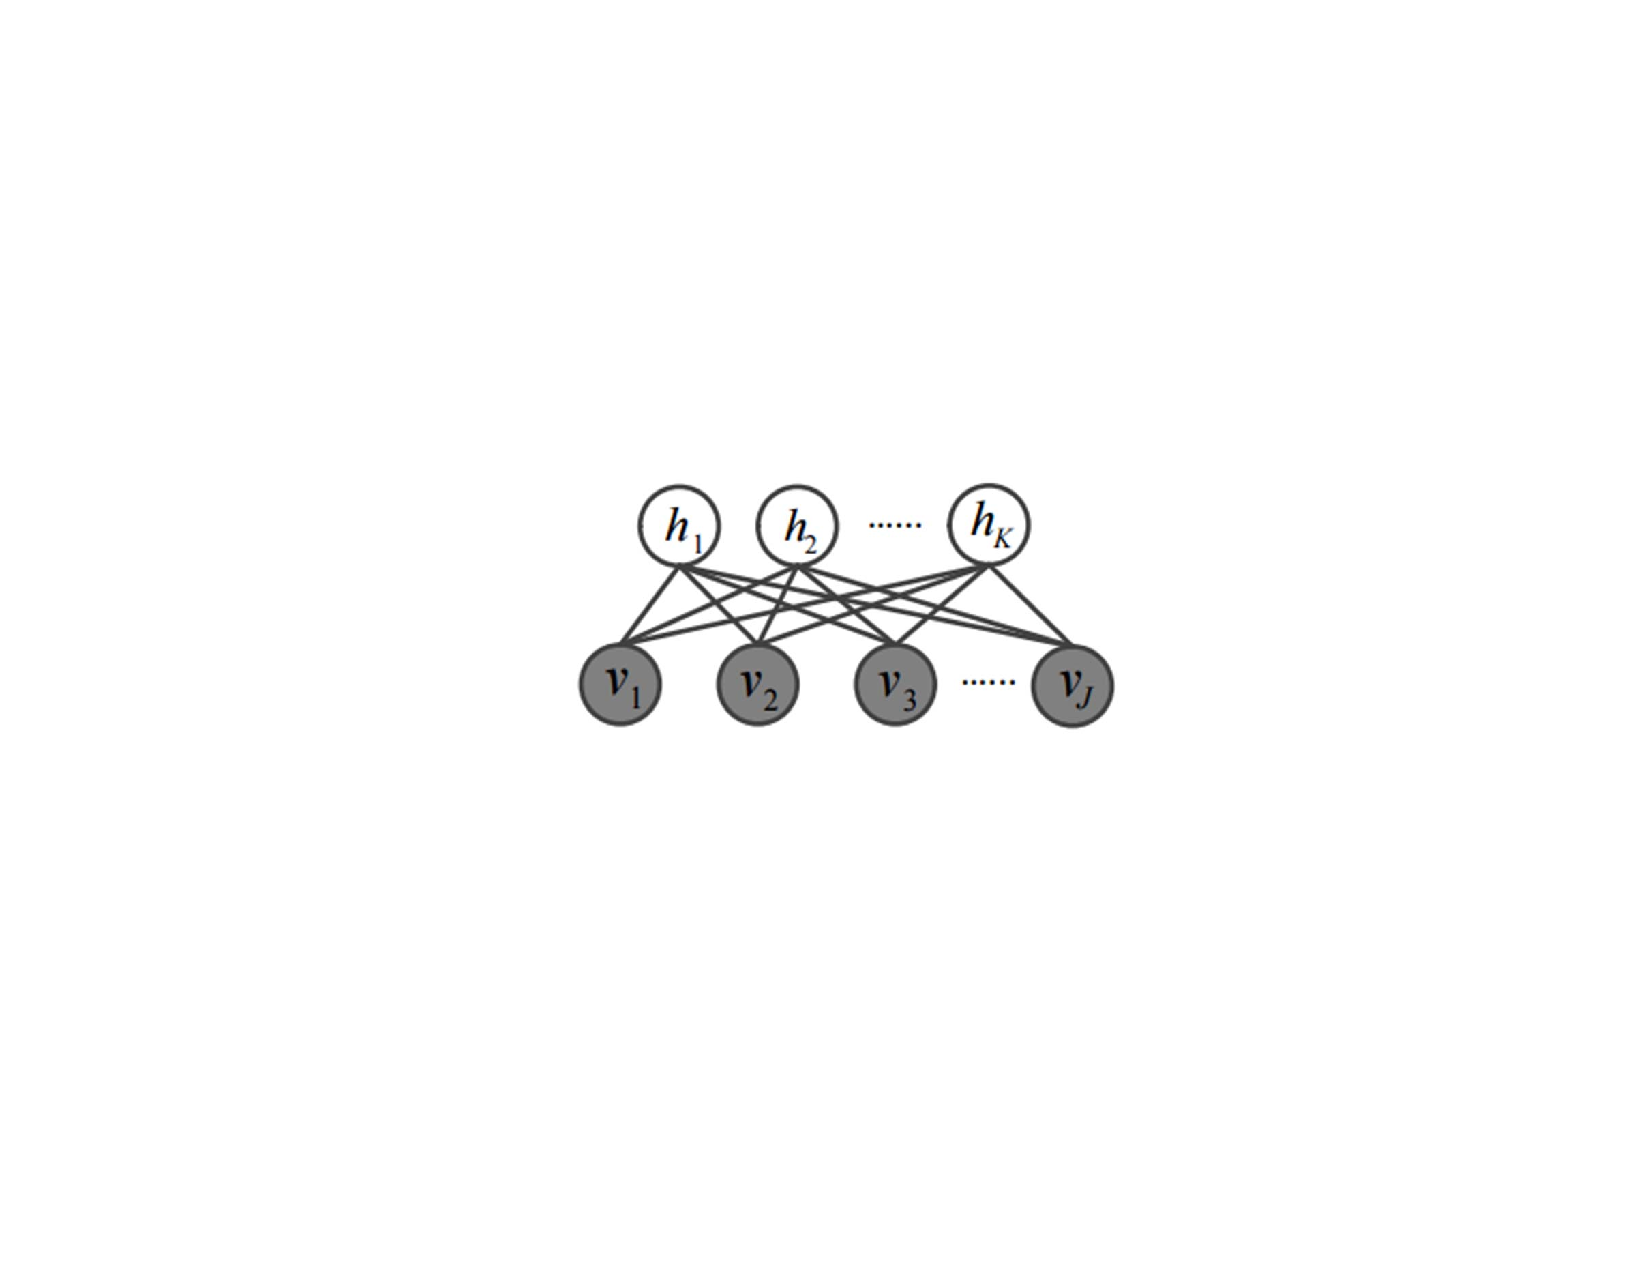
\includegraphics[width=0.4\textwidth]{Figure/rbm} \\
  \caption{A restricted Boltzmann machine.}\label{rbm}
\end{figure}
